% This is samplepaper.tex, a sample chapter demonstrating the
% LLNCS macro package for Springer Computer Science proceedings;
% Version 2.20 of 2017/10/04
%
\documentclass[runningheads]{llncs}
%
\usepackage{xcolor}


\usepackage{graphicx}


\usepackage[utf8]{inputenc} %Together with 'spanish' package, allows you to write accents 

%This package allows the use of accents, the parameter 'es-tabla' writes Tabla instead of 'Cuadro', the parameter es-noindentfirst makes that the first line after each section and subsection is not indented
\usepackage[spanish,activeacute,es-tabla,es-noindentfirst]{babel}

%This package allows you among other things, use as option [H] in tables and figures, which set the object just where you put in the source code.
\usepackage{float}

%This package allows you to write pseudocode, you should read the docummentation to use it properly 
\usepackage{algorithm2e}

%Packages to write math
\usepackage{amssymb}
\usepackage{amsmath}

%permite el formato de múltiple citación agrupada dentro de los corchetes
\usepackage{cite} 

\usepackage{times}
\usepackage{color}

%Package that help to write text that will appear like you write in the final documment
\usepackage{verbatim}

%This package allows you to configure tables and figures
\usepackage{caption}

%Package to customize formats to the tables
\usepackage{booktabs}

%Package to control hiperlinks
\usepackage[breaklinks=true]{hyperref}
\hypersetup{
	colorlinks=true,
	linkcolor=blue,
	filecolor=magenta,      
	urlcolor=blue,
	citecolor=cyan,
}

%Package to stablish the margins of the documment
\usepackage{vmargin}

%A0, A1, ..., A9, B0, B1, ..., B9, C0, ..., C9, USletter, USlegal, and USexecutive
\setpapersize{A4}
%\setmarginsrb{hleftmargini}{htopmargini}{hrightmargini}{hbottommargini}%
%{hheadheighti}{hheadsepi}{hfootheighti}{hfootskipi}

\setmarginsrb{30mm}{25mm}{30mm}{25mm}{6mm}{7mm}{5mm}{15mm}

%También puede utilizar esta sintaxis para establcer los márgenes con el paquete {vmargin}
%\setmargins{3.0cm}       % margen izquierdo
%{1.5cm}                        % margen superior
%{14.5cm}                      % anchura del texto
%{23.42cm}                    % altura del texto
%{10pt}                           % altura de los encabezados
%{1cm}                           % espacio entre el texto y los encabezados
%{0pt}                             % altura del pie de página
%{2cm}         

%Estos paquetes se utilian para escribir psudocódigo, sin embargo en estos momentos se está utilizando el paquete {algorithm2e}
%\usepackage{algpseudocode}
%\usepackage{algorithmicx}
%\usepackage{algorithm}

\definecolor{gray97}{gray}{.97}
\definecolor{gray75}{gray}{.75}
\definecolor{gray45}{gray}{.45}

%Packages to write code in various programming languajes, please, see the docummentation 
\usepackage{listings}
\usepackage{listingsutf8}
\lstset{frame=Ltb,
	framerule=0pt,
	aboveskip=0.5cm,
	framextopmargin=3pt,
	framexbottommargin=3pt,
	framexleftmargin=0.4cm,
	framesep=0pt,
	rulesep=.4pt,
	backgroundcolor=\color{gray97},
	rulesepcolor=\color{black},
	%
	stringstyle=\ttfamily,
	showstringspaces = false,
	basicstyle=\small\ttfamily,
	commentstyle=\color{blue},
	keywordstyle=\bfseries,
	%
	numbers=left,
	numbersep=15pt,
	numberstyle=\tiny,
	numberfirstline = false,
	breaklines=true,
}
\lstnewenvironment{listing}[1][]
{\lstset{#1}\pagebreak[0]}{\pagebreak[0]}

\lstdefinestyle{consola}
{basicstyle=\scriptsize\bf\ttfamily,
	backgroundcolor=\color{gray75},
}
\lstdefinestyle{C}
{language=C,
}
% Used for displaying a sample figure. If possible, figure files should
% be included in EPS format.
%
% If you use the hyperref package, please uncomment the following line
% to display URLs in blue roman font according to Springer's eBook style:
\renewcommand\UrlFont{\color{blue}\rmfamily}

%\renewcommand\Algorithmname{Algoritmo}
\renewcommand\examplename{Ejemplo}
\renewcommand\exercisename{Ejercicio}
\renewcommand\figurename{Fig.}
\renewcommand\keywordname{{\bf T\'erminos Clave:}}
\renewcommand\indexname{Index}
\renewcommand\lemmaname{Lema}
\renewcommand\contriblistname{Lista de colaboradores}
\renewcommand\listfigurename{Lista de Figuras}
\renewcommand\listtablename{Lista of Tablas}
\renewcommand\mailname{{\it Correspondencia para\/}:}
\renewcommand\noteaddname{Note added in proof}
\renewcommand\notename{Nota}
\renewcommand\partname{Parte}
\renewcommand\problemname{Problema}
\renewcommand\proofname{Demostración}
\renewcommand\propertyname{Propiedad}
\renewcommand\propositionname{Proposici\'on}
\renewcommand\questionname{Pregunta}
\renewcommand\remarkname{Remark}
\renewcommand\seename{Ver}
\renewcommand\solutionname{Soluci\'on}
\renewcommand\theoremname{Teorema}
\begin{document}

\section{\centering{Generalidades del Proyecto}}



\subsection{Antecedentes}
La Universidad Linda Vista, cuenta con un grupo de alumnos que financia sus estudios a traves de la venta de publicaciones llamado colportaje, los alumnos salen cada periodo vacacional de invierno y verano a diversos estados de Mexico o el extranjero. El alumno realiza la compra de las publicaciones a la casa editora GEMA, y realiza la venta minorista de manera directa con el cliente, este proceso se realiza a traves de un talonario impreso en papel, en el cual, se registra la informacion de la venta, que consiste entre otros titulo del libro, precio, fecha de entrega y fechas de pago por parte del cliente, etc. Terminada la fase anterior se emite una copia del talonario al cliente y el recibo original queda a resguardo del colportor, para el control de ventas.
Actualmente, no se cuenta con ninguna otra herramienta creada o emitida por la casa editora o por la universidad que permita registrar la informacion comentada anteriormente a traves de una aplicacion que este enfocada a la gestion del colportaje, sin embargo ha sido de interes por parte de los alumnos que esta exista, en virtud de lo manifestado en el cuestionario aplicado a una muestra de 35 colportores universitarios de edades entre los 18 a los 30 años, con el objetivo de obtener información sobre cómo realizan su trabajo y cómo llevan el control de sus ventas, compras y créditos. Los resultados de la encuesta ayudaron a comprender los desafíos y obstáculos que enfrentan los colportores en su trabajo diario y pueden ser utilizados para desarrollar soluciones que los apoyen a gestionar la informacion de ventas de manera digital.

\subsection{Descripción de la empresa}

La Universidad Linda Vista apoya y motiva al estudiante para ser un colportor y financiar de esta manera sus estudios a traves del club KERUSSO S.C. Esta se encuentra ubicada en las instalaciones de la misma universidad con direccion en Ex-Finca Santa Cruz \# 1, 29750 Municipio de Pueblo Nuevo Solistahuacán, Chiapas, Mexico. Este club dispone con una organización interna conformada por estudiantes y empleados y tiene como porposito capacitar a los estudiantes para tener exito en el colportaje, brindandoles herramientas necesarias para ser efectivos en su campo correspondiente.\\
Este club cuenta con una oficina cuya informacion de contacto es la siguiente: Telefono (+52) 961 304 8241 y correo electronico colportores.kerusso@ulv.edu.mx.

\subsection*{Filosofía:}
\begin{itemize}
    \item De nuestros libros y periódicos han de emanar brillantes rayos de luz que han de iluminar al mundo con respecto a la verdad presente.
    \item El Señor ha instituido un plan por el cual muchos alumnos de nuestros colegios pueden aprender lecciones prácticas necesarias para tener éxito en la vida posterior.
    \item Cuando finalizan las clases, habrá oportunidades para que muchos salgan al campo como Colportores evangélicos.
\end{itemize}
\subsection*{Misión: }
Instruir a estudiantes bajo la dirección de Dios, como un ministerio colaborador en el proceso educativo de todo joven.
\subsection*{Visión: }
Distribuir el mensaje de salvación a través de publicaciones adventistas, con jóvenes capaces y dispuestos a alcanzar almas para Cristo en todo México.
\subsection*{Blanco: }
Proclamando las Verdades del Evangelio con las publicaciones hasta que Cristo venga.
\subsection*{Lema: }
Motivados por el Espíritu Santo.
\subsection*{Voto:} 
Colportores estudiantes, unidos por el compromiso de servir a la sociedad, llevando el mensaje de salvación a través de la página impresa.
\subsubsection*{Valores: }
\begin{itemize}
    \item Integridad
    \item Consagración
    \item Fidelidad
    \item Trabajo
    \item Responsabilidad
    \item Lealtad
    \item Liderazgo
\end{itemize}

\subsection{Organizacion  de la Empresa}
\begin{figure}[H]
	\centering\captionsetup{width=0.8\textwidth}
	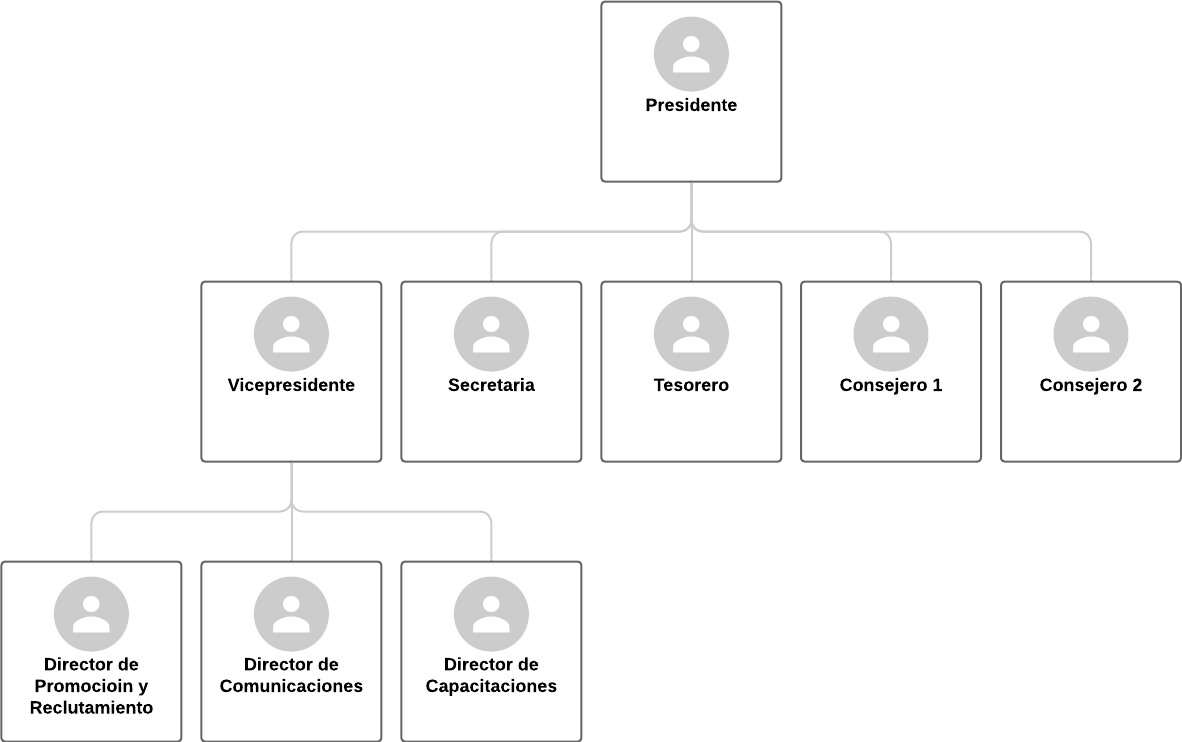
\includegraphics[width=1\textwidth]{figures/Organigrama.png}
	\caption{Organizacion Empresarial de Kerusso} \label{fig1}
\end{figure}


\subsection{Plantemiento del Problema}
Actualmente el club de colportores KERUSSO, gestiona sus ventas por medio de talonarios físicos como ya se ha mencionado, este sistema si bien es efectivo y funcional, es un sistema que tiene muchos inconvenientes para los colportores, tales como:
\begin{itemize}
    \item Acumulación de recibos por cada pedido complicando la gestión de las ventas y pedidos. 
    \item Riesgo de extravio de los recibos, en virtud de no existir un respaldo de esta información.
    \item La gestión de cobros y pedidos se hace compleja y tediosa.
    \item No existe un sistema que notifique al colportor sobre la fecha de entrega y cobro de los materiales, existiendo retrasos en la entrega del pedido y del cobro del producto por parte del colportor.
\end{itemize}
En vista de lo anterior, se ha identificado una necesidad por parte de los colportores y el club KERUSSO, de crear una herramienta que optimice los procesos, disponiendo de una alternativa para una mejor gestión del colportaje, haciendo uso de las tecnologías de la informacion.

\subsection{Objetivos del Proyecto}
\subsection*{Objetivo General}
Desarrollar un software que permita optimizar los procesos de gestion del colportaje de los estudiantes del club de colportores Kerusso.
\subsection*{Objetivos Especificos}
\begin{itemize}
    \item Obtener y analizar los requerimientos para el desarrollo del software.
    \item Diseñar las interfaces graficas y logicas del software.
    \item Codificar los modulos del software de acuerdo a los requerimientos y diseños.
    \item Realizar pruebas funcionales y de calidad de software.
    \item Implementar el software para su produccion.
    \item Capacitar a los usuarios finales en el uso del software.
\end{itemize}

\subsection{Justificacion}

La constante necesidad de estar actualizados con las tecnologías actuales y aprovechar esos recursos es algo fundamental actualmente para obetener el mayor rendimiento y optimización en nuestro trabajo. Es por eso que, con base en las respuestas del cuestionario y las problemáticas mencionadas anteriormente, se observa la necesidad de desarrollar un sistema para mejorar el proceso de gestión de ventas y pedidos en el colportaje estudiantil. Por lo tanto, se propone la creacion e implementación de una herramienta digital de gestión de ventas y pedidos para los colportores. Al realizar este sistema, el colportor se vera beneficiado en una menor inversion de tiempo en el registro y control de ventas y pedidos asi como una reduccion de uso de papel y brindar una mejor experiencia de colportaje. A partir de este sistema, podrian desarrollarse herramientas que beneficien y mejoren la supervicion y consulta de ventas por parte de los colportores de manera centralizada y contar con informacion que permita tomar desiciones para futuras campañas de colportaje desde la directiva del club Kerusso.


\subsection{Alcances y Limitaciones}
El sistema de gestión de colportaje permitirá controlar las ventas, pedidos, clientes, creditos y catalogo de libros disponibles, y como una primera implementacion de este, se limitara a la informacion que dispone el club de colportores Kerusso. Además, el colportor asociado podrá supervisar y consultar las ventas de sus colportores asignados.

\newpage


\end{document}
